
\documentclass[letterpaper,11pt]{texMemo} % Set the paper size (letterpaper, a4paper, etc) and font size (10pt, 11pt or 12pt)
\usepackage{parskip} % Adds spacing between paragraphs
\setlength{\parindent}{15pt} % Indent paragraphs
\usepackage{amsmath,amsthm} 
\usepackage{amsfonts} 


%----------------------------------------------------------------------------------------
%	MEMO INFORMATION
%----------------------------------------------------------------------------------------

%\memoto{James Smith} % Recipient(s)

\memofrom{Ben Rapone} % Sender(s)

\memosubject{Tree Canopy Model} % Memo subject

\memodate{\today} % Date, set to \today for automatically printing todays date

\logo{\includegraphics[width=0.3\textwidth]{wsumath.jpg}} % Institution logo at the top right of the memo, comment out this line for no logo

%----------------------------------------------------------------------------------------

\begin{document}

\maketitle % Print the memo header information

%----------------------------------------------------------------------------------------
%	MEMO CONTENT
%----------------------------------------------------------------------------------------

\section{Objective}

\begin{enumerate}
\item[$\bullet$] Long Term: Identify key ecological factors that allow for successful modelling of tree canopy development using optimization (preferably linear) methods. 
\item[$\bullet$] Short Term: Develop a formulation that allows for flexible programming, and ease of incorporation of potential key factors. 
\end{enumerate}


\section{Theory and Methodology}

To expedite the process of choosing the right formulation it became necessary to consider a lower dimensional form of the problem. By modelling a "cross-section" of the canopy the initial problem now becomes two dimensional in nature, and is what will be the focus of what follows. All efforts and results have kept in mind the need to generalize to the three dimensional case. Programming using the Python language was determined to provide the most flexibility for coding and interface with optimization and meshing software (CPlex and Triangle respectively). 

\noindent The running ecological hypothesis is that tree canopy development is highly influenced by the need to optimize exposure to sunlight. From an optimization standpoint this translates to an objective function where the goal is to maximize the sum of the edge lengths that trace the "cross-section" of the canopy. In order to produce a continuous edge-path without loops or multiple use of edges inspiration was taken from the Miller-Tucker-Zemlin (MTZ) formulation used most commonly in conjunction with the travelling salesman problem. Briefly the basic formulation is as follows: 

\begin{align*}
\intertext{ Maximize sum of edge distances "$x_{ij}$" without considering the node positions $U_j$s } \\
\max \ \ &\sum x_{ij}+0*\sum U_j \\
\intertext{ Subject to:}\\
\intertext{Outgoing Restraint: Can only leave a node at most 1 time } \\
& \sum\limits_{j} x_{ij}\leq 1 \\
\intertext{Incoming Restraint: Number of times you enter a node is $\leq$ number of times you leave a node. } \\
& \sum_i x_{ij}-\sum_j x_{ij}\leq 0 \\
\intertext{Starting Node Restraint: Must leave the first node of original edge and cannot enter it. } \\
& \sum\limits_{j} x_{1j}=1\quad\quad \sum\limits_{i} x_{i1}=0 \\
\intertext{Ending Node Restraint: Must enter the last node of original edge and cannot leave it. } \\
&\sum\limits_j x_{16,j}=0\quad\quad \sum\limits_i x_{i,16}=1 \\
\intertext{Last Node Place Value Restraint: All Nodes are assigned a place value less then that of the place value of the last node in the original edge. } \\
& U_i-U_{16}\leq -1 \\
\intertext{Original Edge Restraint: Cannot use any edge along bottom edge} \\
& x_{ij}=0 \\
\intertext{Subtour Restraint: No cycles (loops)} \\
& U_i-U_j\leq n(1-x_{ij})-1 \text{ where } n=MaxNumEdges \\
\intertext{Max Edges Restraint: Sets a limit on the highest value the place value of the last node can take } \\
& U_{\text{EndNode}}\leq MaxNumEdges 
\intertext{Node Positions are at least 1 if used} \\
& \sum\limits_{j}x_{ij}-U_i\leq 0 
\end{align*}

This formulation by itself produces a scattered and zigzag like pattern that maximizes total space
available without any additional consideration. An example of this formulation on a eleven by eleven grid is shown below.

\begin{center}
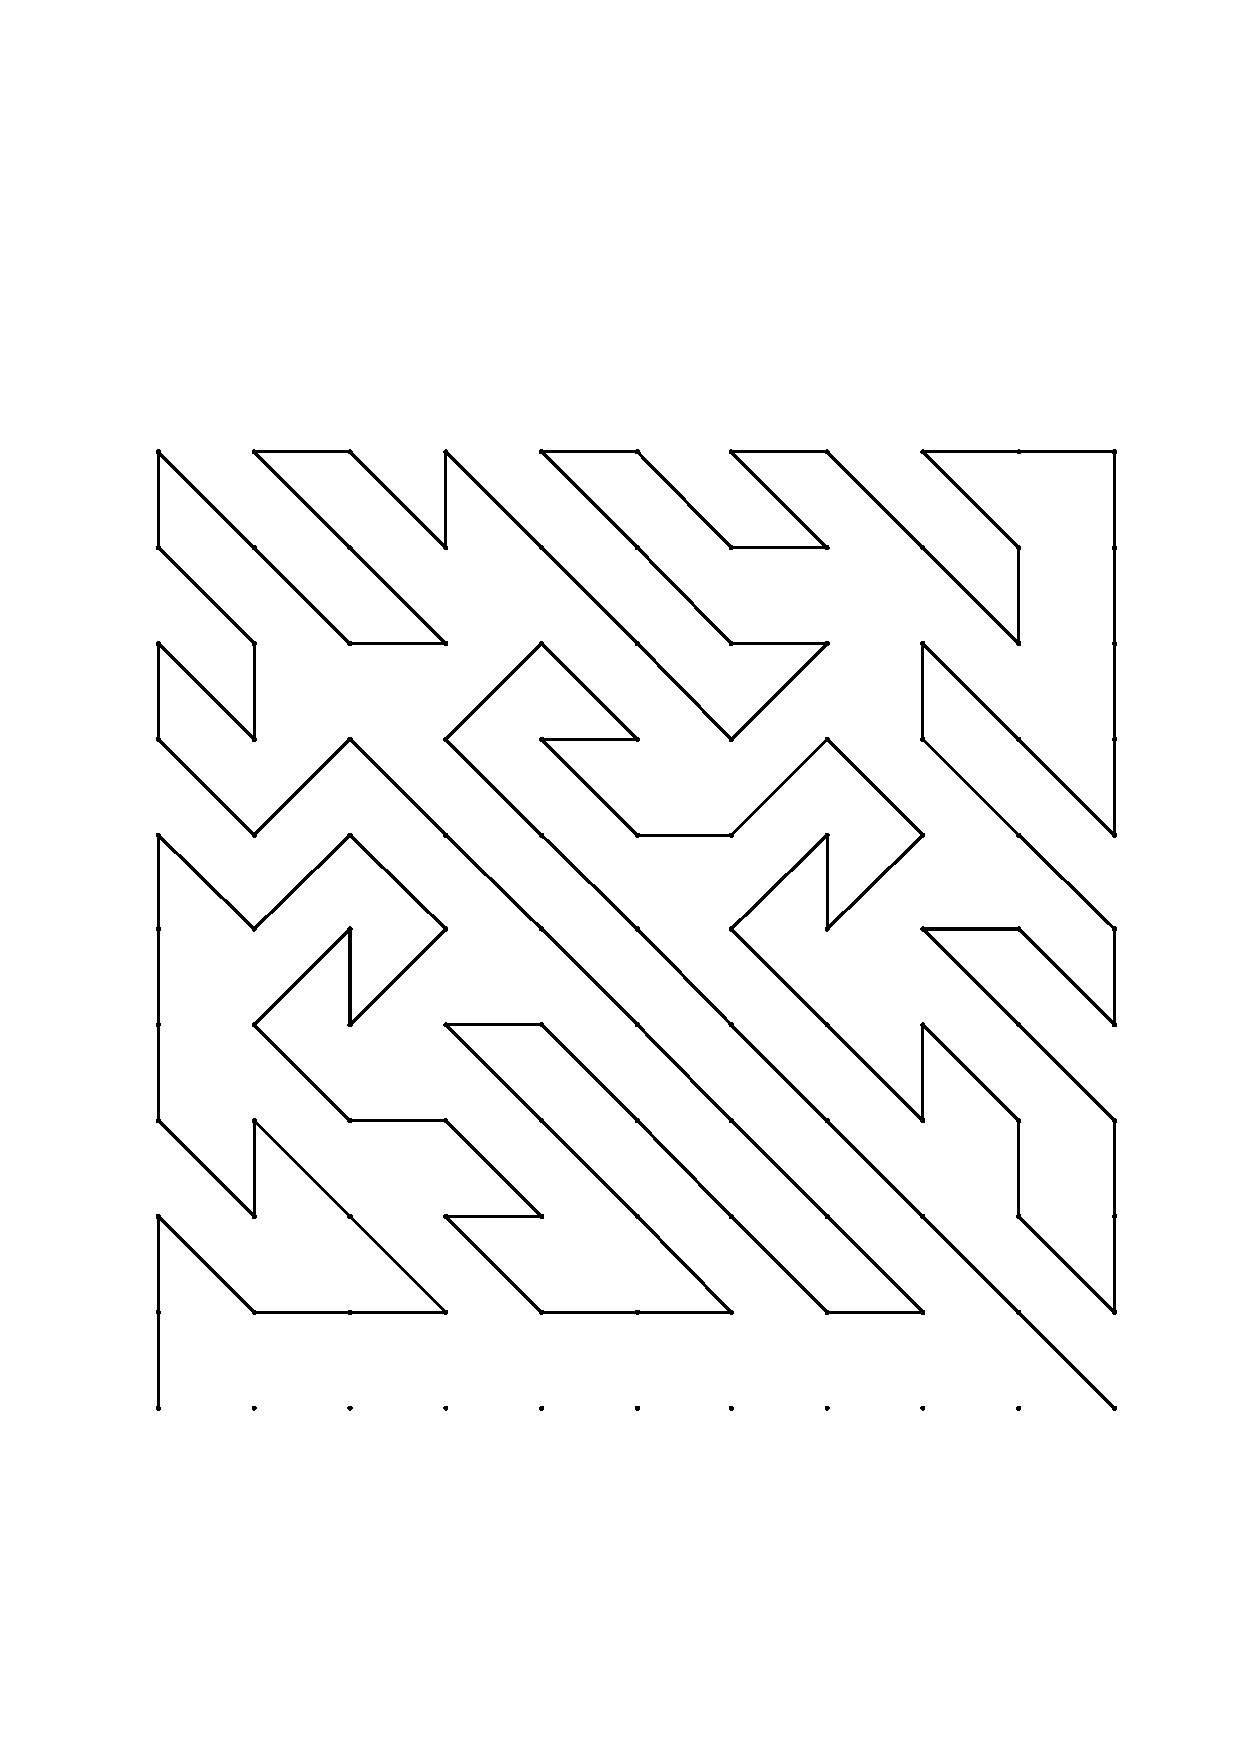
\includegraphics[scale=0.35]{OptimalLimitless111EdgesUsed.pdf}
\end{center}

\section{Progress and Examples}

Although the basic formulation does produce interesting results, it was abundantly clear that further "ecological" restrictions are needed. This provided an opportunity, and as it happens a necessary one, to test the flexibility of the programming. The following example uses a twelve by twelve grid with 576 uniformly dispersed nodes. The objective is to minimize the "overlap" or redundancy of edges along paths of sun light. Using the assumption that the sun is mostly overhead we can group the edges into very basic, distinct classes as shown in the plot below. The colors represent the different classes. 

\begin{center}
\includegraphics[scale=1]{Daylight.png}
\end{center}

By limiting the amount of edges in any one class the amount of overlap in each class can be moderated. Additionally, because of the overlap of the classes the program is motivated to choose as few edges in multiple classes as possible.
To this end the following restrictions were added after the edges were classified.

\begin{align*}
\intertext{Side/Horizontal edge class Constraint}\\
& \sum\limits_{x_{ij}\in\text{Side Class}} x_{ij}\leq\text{ SideCap} \\
\intertext{Left Diagonal edge class Constraint}\\
& \sum\limits_{x_{ij}\in\text{Left Diagonal Class}} x_{ij} \leq\text{ DiagCap}\\
\intertext{Right Diagonal edge class Constraint}\\
& \sum\limits_{x_{ij}\in\text{Right Diagonal Class}} x_{ij} \leq\text{ DiagCap} \\
\intertext{Outside vertical edge class Constraint}\\
& \sum\limits_{x_{ij}\in\text{Outside Vert Class}} x_{ij} \leq\text{ OutVertCap}\\
\intertext{Inside vertical edge class Constraint}\\
& \sum\limits_{x_{ij}\in\text{Inside Vert Class}} x_{ij} \leq\text{ InVertCap}\\
\end{align*}

There are many potential avenues to move forward such as creating more classes, thinner classes,
or even utilizing the idea of classes to model energy or weight distribution. However, with more
ecological insight it may prove easier to determine which factors are more effective.

The following are the results of running models with various caps as described under each image. 

\begin{center}
\includegraphics[scale=0.25]{24X18S30D20TO10TI.pdf} \  \includegraphics[scale=0.25]{24X18S30D20TO20TI.pdf} \\
Fig 1 (left): SideCap(SC)=18, DiagCap(DC)=20, OutVertCap(OV)=20, InVertCap(IV)=10\\
Objective: Minimize all edges in every class. \\
Fig 2 (right): SC=18, DC=30, OV=20, IV=20 \\
Objective: Slightly increase diagonal while keeping all other classes at a minimum. \\
\includegraphics[scale=0.25]{24X18S30D30TO20TI.pdf} \  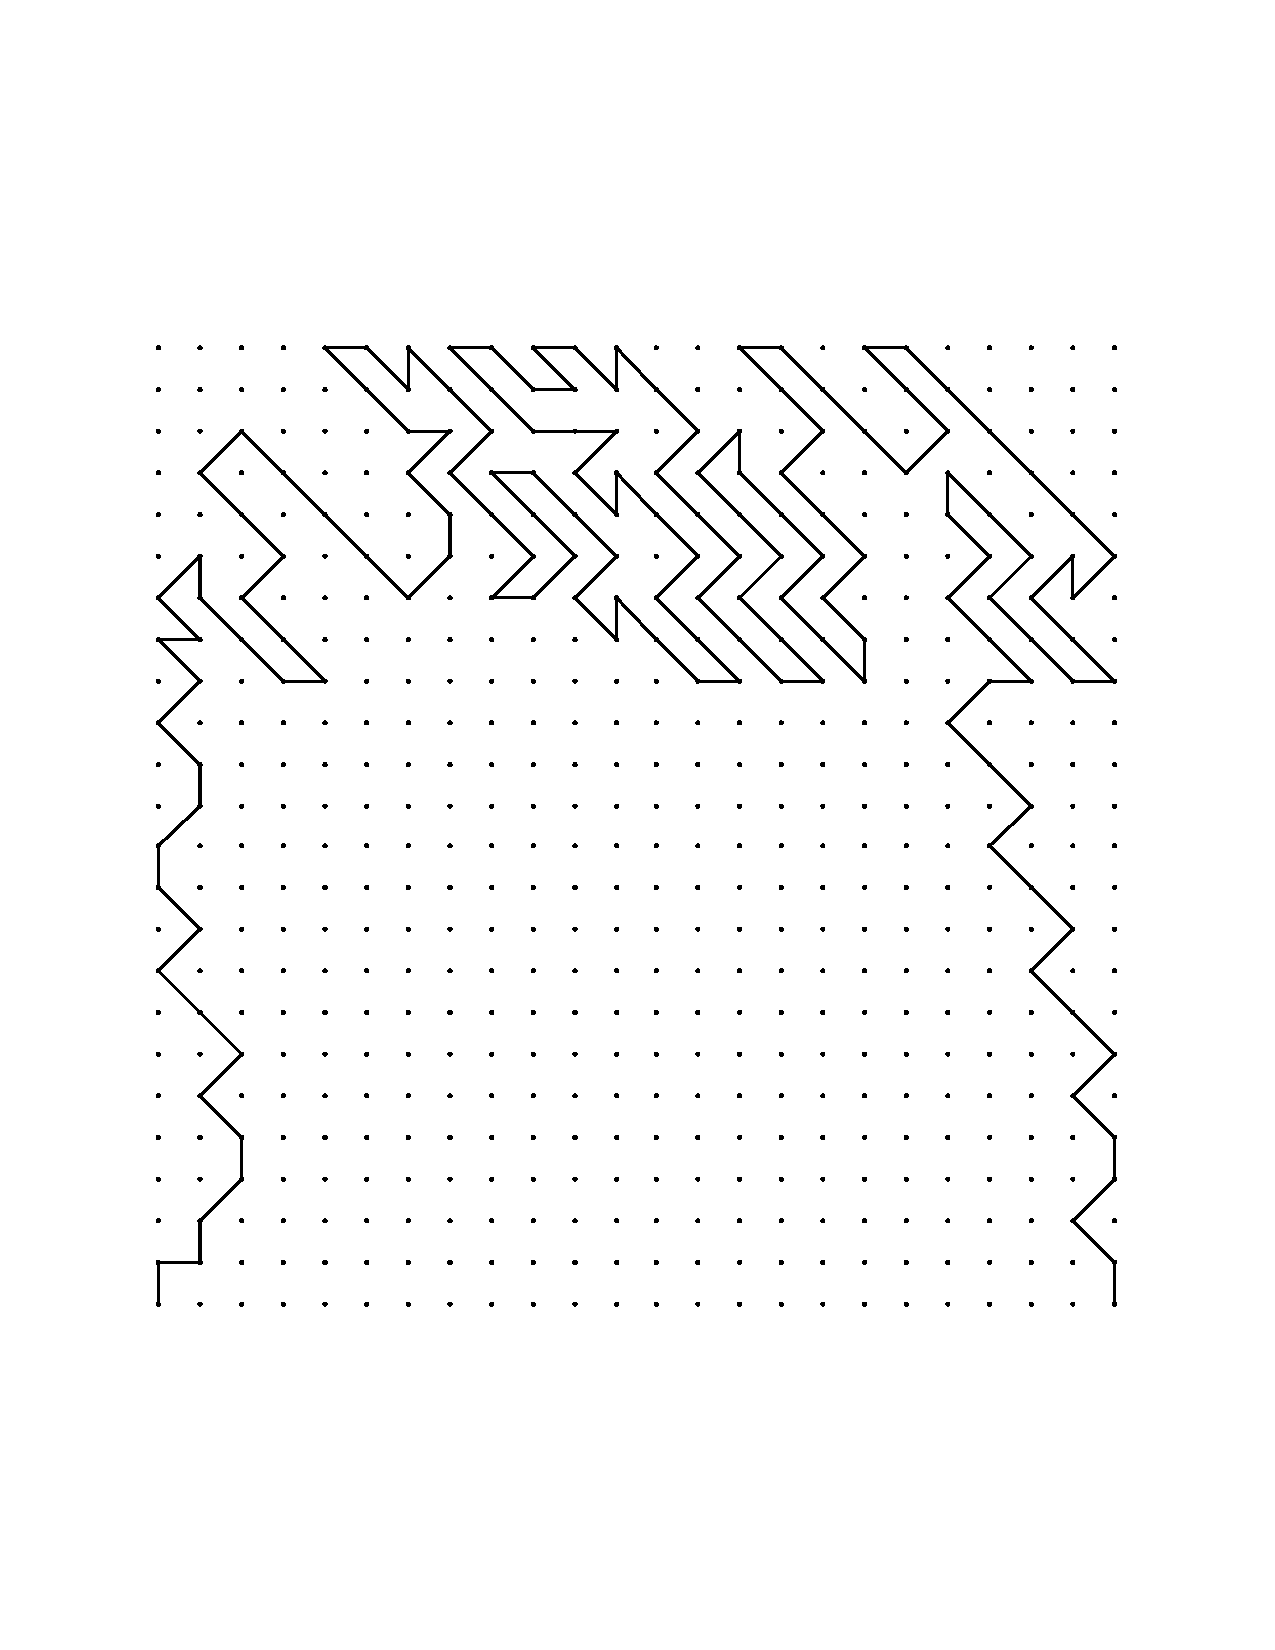
\includegraphics[scale=0.25]{24X18S30D40TO40TI.pdf} \\
Fig 3: SC=18, DC=30, OV=30, IV=20 \\
Obective: Increase the availability of the outside vertical edges in Fig 2 in order to see if edges will spread more evenly. \\
Fig 4: SC=18, DC=30, OV=40, IV=40 \\
Objective: Keep Sie constraint at a minimum, diagonals with a little freedom, while dramatically increasing all verticals to see if more horizontal edges would be used.\\
\includegraphics[scale=0.25]{24X18S30DTO30TI40.pdf} \  \includegraphics[scale=0.25]{24X18S35D40TO40TI.pdf} \\
Fig 5: SC=18, DC=30, OV=30, IV=40 \\
Objective: Concentrate the edges in Figure 4 to the inside vertical edges. \\
Fig 6: SC=18, DC=35, OV=40, IV=40\\
Objective: Increase the diagonals from Figure 4 in order to fill in corners if possible. \\
\includegraphics[scale=0.25]{24X20S40D40TO30TI.pdf} \  \includegraphics[scale=0.25]{24X20S50D20TO20TI.pdf} \\
Fig 7: SC=20, DC=40, OV=40, IV=30 \\
Objective: Test if we get similar results as in Fig. 3 by keeping the same ratio and increasing the caps. \\
Fig 8: SC=20, DC=50, OV=20, IV=20 \\
Objective: Will drastically increasing the diagonals but minimizing the verticals cause more diagonal edges to be chosen.\\
\includegraphics[scale=0.25]{24X20S50D30TO30TI.pdf} \  \includegraphics[scale=0.25]{24X20S50D30TO40TI.pdf} \\
Fig 9: SC=20, DC=50, OV=30, IV=30\\
Objective: Expanding on Fig. 8 by loosening all the vertical restrictions. \\
Fig 10: SC=20, DC=50, OV=30, IV=40 \\
Objective: Modify Fig. 9 by increasing the inside vertical restraints and comparing this to Fig. 5.\\
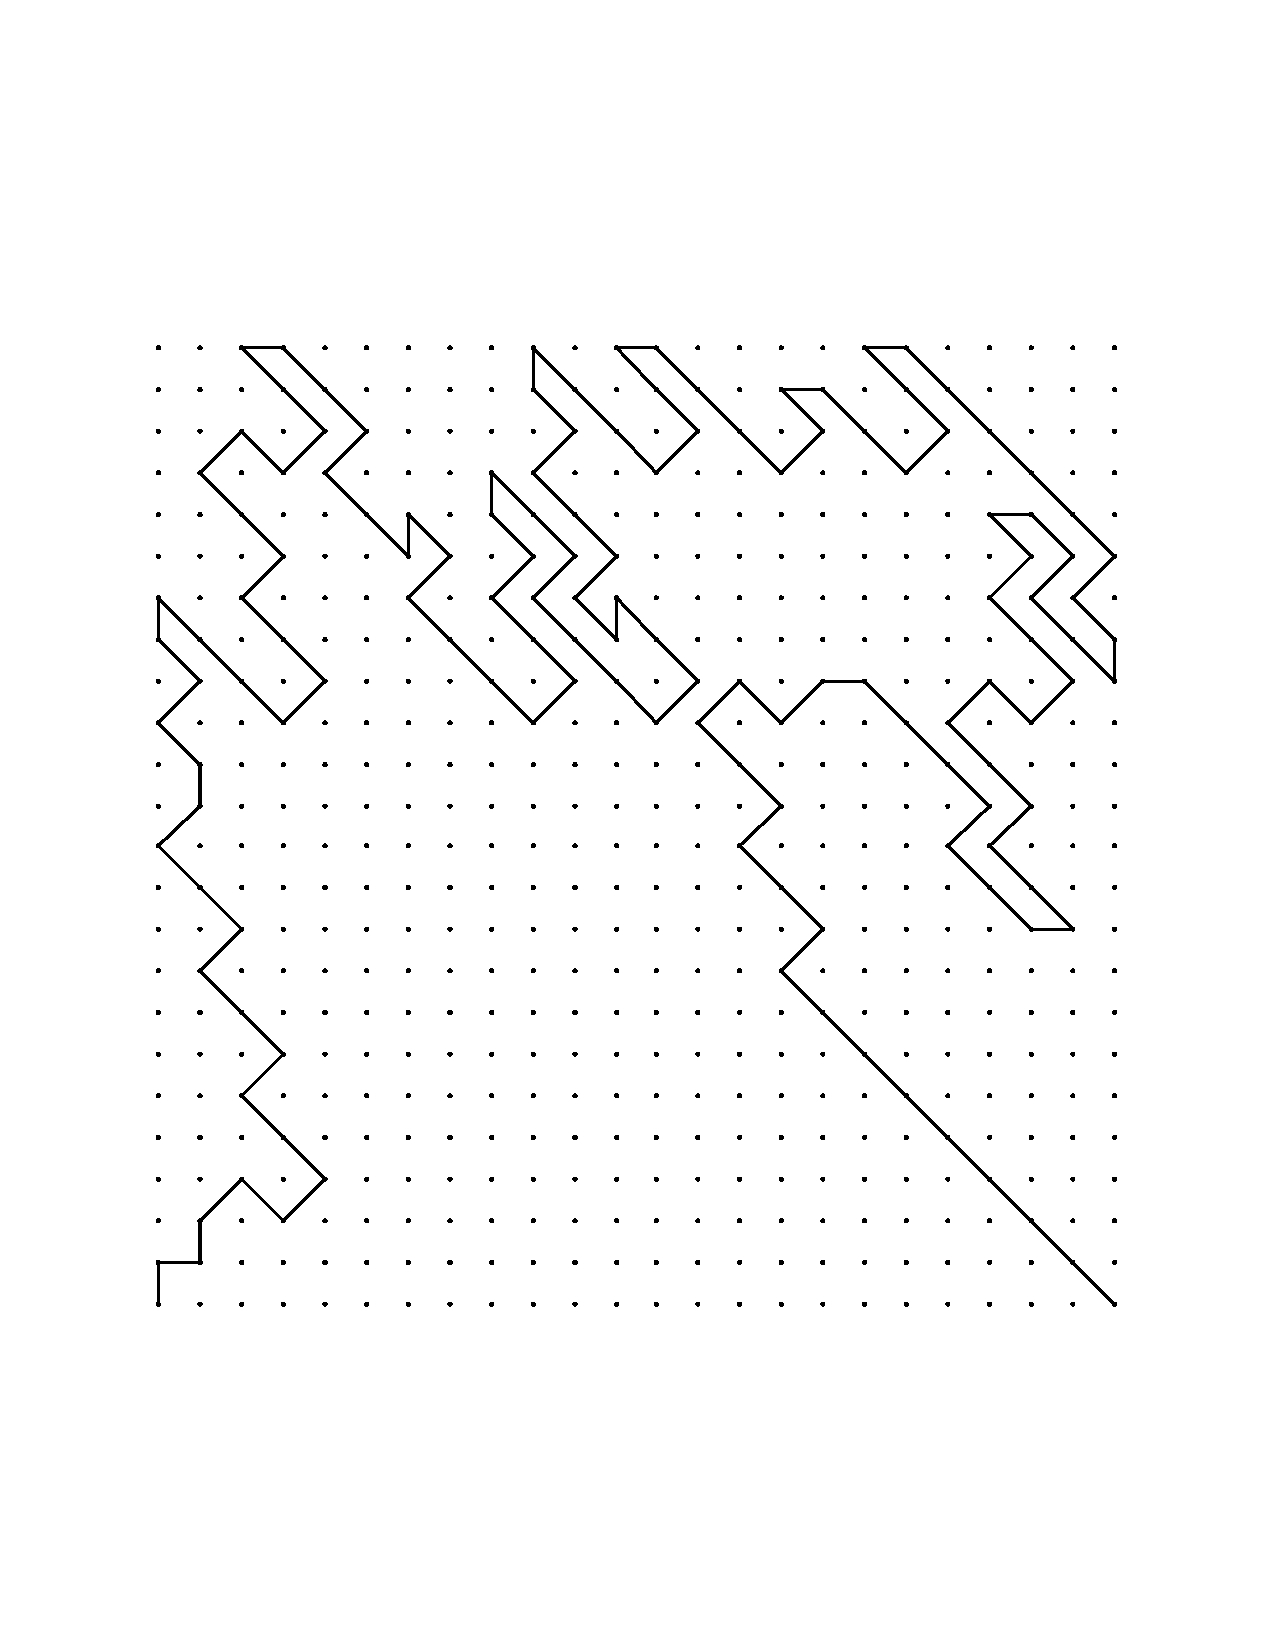
\includegraphics[scale=0.25]{24X20S50D40TO30TI.pdf} \  \includegraphics[scale=0.25]{24X20S50D50TO20TI.pdf} \\
Fig 11: SC=20, DC=50, OV=40, IV=30\\
Objective: Expanding on Fig. 9 by increasing the diagonal restraints and comparing this to FIg. 7. \\
Fig 12: SC=20, DC=50, OV=50, IV=20\\
Objective: Drastically restricting the inside verticals to see if this would push the graph into the corners.\\
\includegraphics[scale=0.25]{24X30S40D30TO30TI.pdf} \  \includegraphics[scale=0.25]{24X30S50D30TO20TI.pdf} \\
Fig 13: SC=30, DC=40, OV=30, IV=30\\
Objective: How does increasing the side constraints effect model constraints. \\
Fig 14: SC=30, DC=50, OV=30, IV=20\\
Objective: Will decreasing the inside vertical constraints and increasing the diagonal constraint to force more edges in the side class to be used.\\
\end{center}

\section{Brief Discussion}
There are many potential avenues to expand such as creating more classes, thinner classes, or even utilizing the idea of classes to model energy or weight distribution. However, with more ecological insight it may prove easier to determine which factors are more effective. 




%----------------------------------------------------------------------------------------

\end{document}